\subsubsection{Registracija kandidata}
\label{subsubsec:registracija}
\begin{itemize}
  \item \textbf{Kratak opis}: Da bi kandidat mogao da se uloguje na svoj nalog i vidi svoje podatke, 
  nepohodno je da dobije potvrdu da je upisan u auto školu, kao i nepohodan ID i lozinku za logovanje.
  \item \textbf{Učesnici}:
  \begin{itemize}
    \item Kandidat - korisnik koji se registruje u auto školu.
    \item Administrator sistema - korisnik koji unosi informacije o kandidatu u bazu.
    \item Administrativni radnik - korisnik koji ažurira spisak kandidata.
  \end{itemize}
  \item \textbf{Preduslovi}:
    \begin{itemize}
    \item  Kandidat je popunio online prijavu.
    \item  Kandidat ispunjava uslove za upis.
    \end{itemize}
  \item \textbf{Postuslovi}:
      \begin{itemize}
      \item Kandidat je evidentiran u sistemu.
      \item Kandidat može da se prijavi na sistem.
      \item Sistem je u funkciji.
      \end{itemize}
  \item \textbf{Osnovni tok}:
      \begin{enumerate}
        \item Administrator sistema prima informacije o novom kadnidatu.
        \item Administrator sistema unosi novog korisnika u bazu podataka.
        \item Sistem čuva unete podatke.
        \item Sistem šalje mejl novom kandidatu sa potvrdom o registraciji i podacima.
        \item Kandidat dobija mejl sa potvrdom o registraciji i podacima.
        \item Sistem šalje mejl administrativnom radniku da je uspešno dodao novog kanidata.
        \item Administrativni radnik prima mejl da je kandidat dodat u bazu.
        \item Administrativni radnik ažurira spisak prijavljenih kandidata dodavanjem novog kadnidata.    
      \end{enumerate} 

      \newpage
  \item \textbf{Alternativni tokovi}:
      \begin{itemize}
        \item A1. \textbf{Kandidat nije dobio mejl sa ID-jem i šifrom za pristupanje svom nalogu.}
        Ukoliko u koraku 5 kandidat nije dobio mejl, administrator sistema zahteva od sistema da ponovo pošalje mejl. Proces se nastavlja u koraku 4. osnovnog toka.
        \item A2. \textbf{Administrativni radnik nije dobio potvrdu o dodavanju novog kandidata.}
        Ukoliko u koraku 7 administrativni radnik nije dobio potvrdu o dodavanju novog kandidata, mejl mu se ponovo šalje tj. proces se nastavlja od 6. koraka osnovnog toka.
      \end{itemize}


  \item \textbf{Specijalni zahtevi}:\newline
  Podaci koji se prosleđuju kandidatu putem mejla su njegov ID i lozinka u bazi, kako bi mogao da se uloguje.
\end{itemize}

\begin{figure}[H]
  \begin{center}
      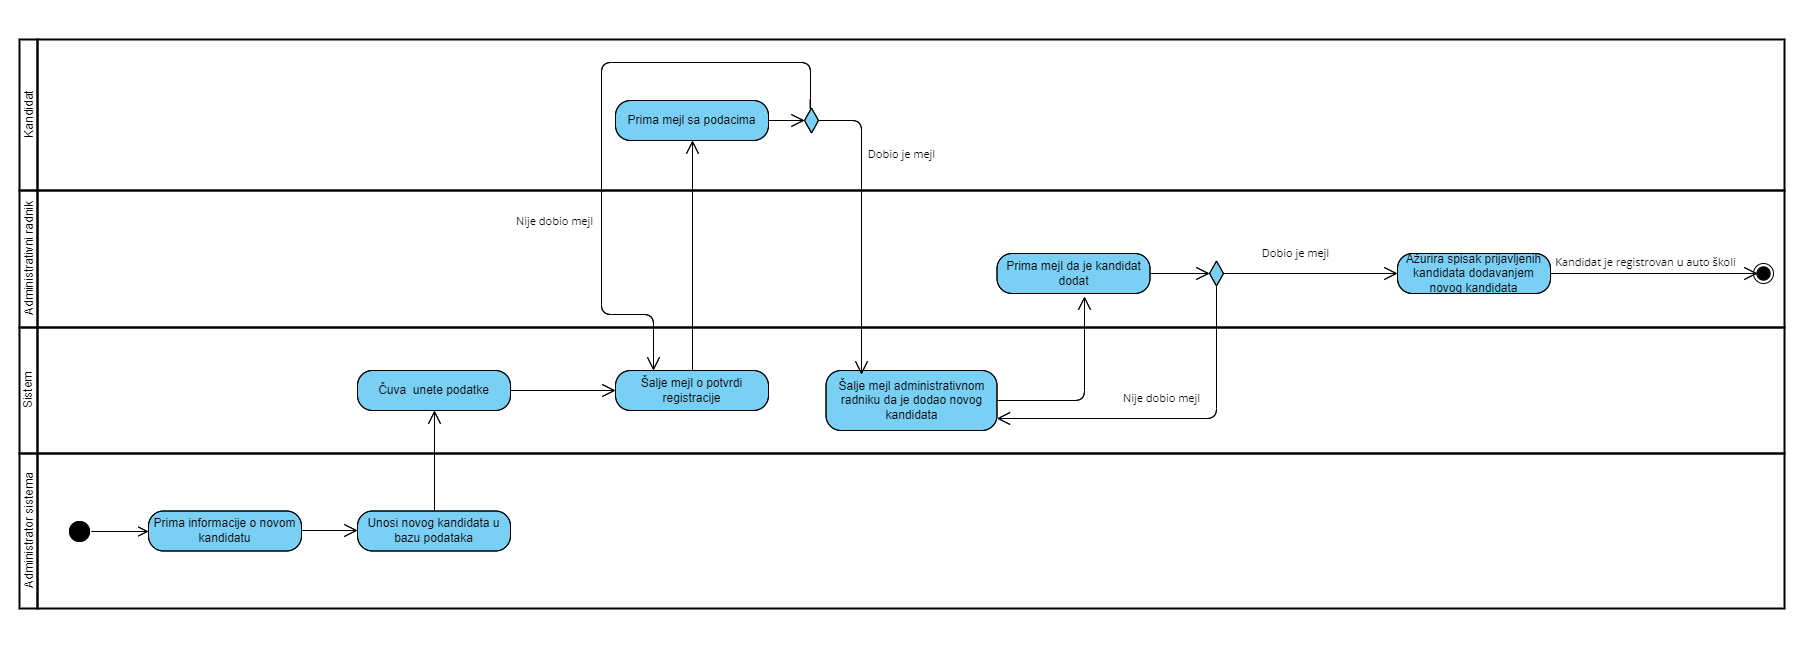
\includegraphics[width=140mm, height=70mm]{Diagrams/dijagram_aktivnosti_registracija_kandidata.png}
  \end{center}
  \caption {Dijagram aktivnosti - Registracija kandidata}
  \label{activity_registracija}

\end{figure}

